% !TeX program = xelatex
\documentclass[12pt,letterpaper]{article}

\usepackage[margin=1in]{geometry}
\usepackage{graphicx}
\usepackage{float}
\usepackage{hyperref}
\usepackage{xcolor}
\usepackage{minted}
\usepackage{fontspec}
\usepackage{xeCJK}
\usepackage{booktabs}
\usepackage{longtable}
\usepackage{placeins}
\setCJKmainfont{AppleGothic} 
\setCJKmonofont{AppleGothic}
% -------------------------------------

\definecolor{backcolour}{rgb}{0.95,0.95,0.92}

\begin{document}
	
\begin{center}
	{\LARGE \textbf{The Nexus of Marriage and Fertility}\par}
	\vspace{0.3em}
	{\LARGE \textbf{in South Korea}\par}
	\vspace{1.5em}
	
	{\large Sein Kim (ID: 25358755)\par}
	\vspace{1.0em}
	
	{\small Data Visualization Final Project | Spring 2026\par}
\end{center}
\vspace{2.0em}
	
	\tableofcontents
	\newpage
	
	\section{Executive Summary}
	Analysis of longitudinal and cross-sectional data highlights a notable spatial mismatch in South Korea’s fertility patterns. The visualizations suggest a pattern that can be interpreted as a “Youth Black Hole” phenomenon: while the childbearing population (ages 20–39) is most concentrated in Seoul and metropolitan hubs, these regions paradoxically record the lowest fertility rates in the nation. A regression-based scatter analysis shows a negative correlation between regional youth share and fertility. Furthermore, indexing analysis suggests that the fertility decline appears closely associated with declining marriage rates, which follows a parallel downward trajectory. The results highlight the importance of considering regional concentration and urban dynamics when discussing Korea’s fertility decline.
	
	\section{Background and Data Summary}
	This project performs a multi-dimensional analysis by integrating three core datasets extracted from the Korean Statistical Information Service (KOSIS). To ensure data integrity, several  processes were conducted, including indexing (rebasing) and the derivation of new demographic variables.
	
	\subsection{Data Sources and Processing}
	
	\begin{enumerate}
		\item \textbf{Total Fertility Rates (TFR) for Provinces (2015--2024)} \\
		\textbf{Contents:} Contains TFR and ASFR for 17 administrative provinces. \\
		I processed the raw data to calculate the absolute drop and percentage change over the decade. This allows for an assessment of whether the decline is a localized or nationwide phenomenon.
		
		\begin{table}[H]
			\centering
			\caption{Descriptive Statistics: Provincial Fertility Change (2015--2024)}
			\label{tab:tfr_change_summary}
			\resizebox{\textwidth}{!}{%
				\begin{tabular}[t]{llllllll}
					\toprule
					& Unique & Missing Pct. & Mean & SD & Min & Median & Max\\
					\midrule
					tfr\_2015 & 16 & 0 & 1.36 & 0.20 & 1.00 & 1.35 & 1.89\\
					tfr\_2024 & 16 & 0 & 0.82 & 0.11 & 0.58 & 0.82 & 1.03\\
					fertility\_drop & 17 & 0 & 0.54 & 0.11 & 0.42 & 0.52 & 0.86\\
					fertility\_drop\_pct & 17 & 0 & -39.59 & 3.50 & -45.69 & -40.04 & -32.19\\
					\bottomrule
			\end{tabular}}
		\end{table}
		
		\item \textbf{Vital Statistics of Korea (Time-Series)} \\
		\textbf{Contents:} National-level crude marriage rates and fertility rates. \\
		To compare indicators with different units, I performed \textbf{indexing (rebasing)} by setting 2015 values to 100. This process reveals the relative speed of decline between marriage and childbirth.
		
		\begin{table}[H]
			\centering
			\caption{Descriptive Statistics: National Marriage and Fertility Time-Series}
			\label{tab:vital_summary}
			\resizebox{\textwidth}{!}{%
				\begin{tabular}[t]{llllllll}
					\toprule
					& Unique & Missing Pct. & Mean & SD & Min & Median & Max\\
					\midrule
					fertility\_rate & 10 & 0 & 0.92 & 0.18 & 0.72 & 0.88 & 1.24\\
					marriage\_rate & 9 & 0 & 4.62 & 0.77 & 3.70 & 4.55 & 5.90\\
					fertility\_index & 10 & 0 & 74.66 & 14.60 & 58.19 & 70.82 & 100.00\\
					marriage\_index & 9 & 0 & 78.31 & 13.03 & 62.71 & 77.12 & 100.00\\
					\bottomrule
			\end{tabular}}
		\end{table}
		
		\item \textbf{Resident Population by Administrative Division (2024)} \\
		\textbf{Contents:} Regional population distribution by age groups. \\
		I derived the \textbf{``Youth Share (\%)"} variable by aggregating the population aged 20--39 and dividing it by the total regional population. This variable is central to analyzing the ``Spatial Mismatch" paradox.
		
		\begin{table}[H]
			\centering
			\caption{Descriptive Statistics: Regional Youth Share and TFR (2024)}
			\label{tab:youth_share_summary}
			\resizebox{\textwidth}{!}{%
				\begin{tabular}[t]{llllllll}
					\toprule
					& Unique & Missing Pct. & Mean & SD & Min & Median & Max\\
					\midrule
					youth\_share & 17 & 0 & 23.34 & 2.83 & 19.09 & 23.13 & 29.65\\
					tfr\_2024 & 16 & 0 & 0.82 & 0.11 & 0.58 & 0.82 & 1.03\\
					\bottomrule
			\end{tabular}}
		\end{table}
	\end{enumerate}
	
	\FloatBarrier
	
	\section{Individual Figures and Analysis}
	
\subsection{Figure 1: Spatial Mismatch Between Youth Concentration and Fertility (The Spatial Paradox)}
	\begin{figure}[H]
		\centering
		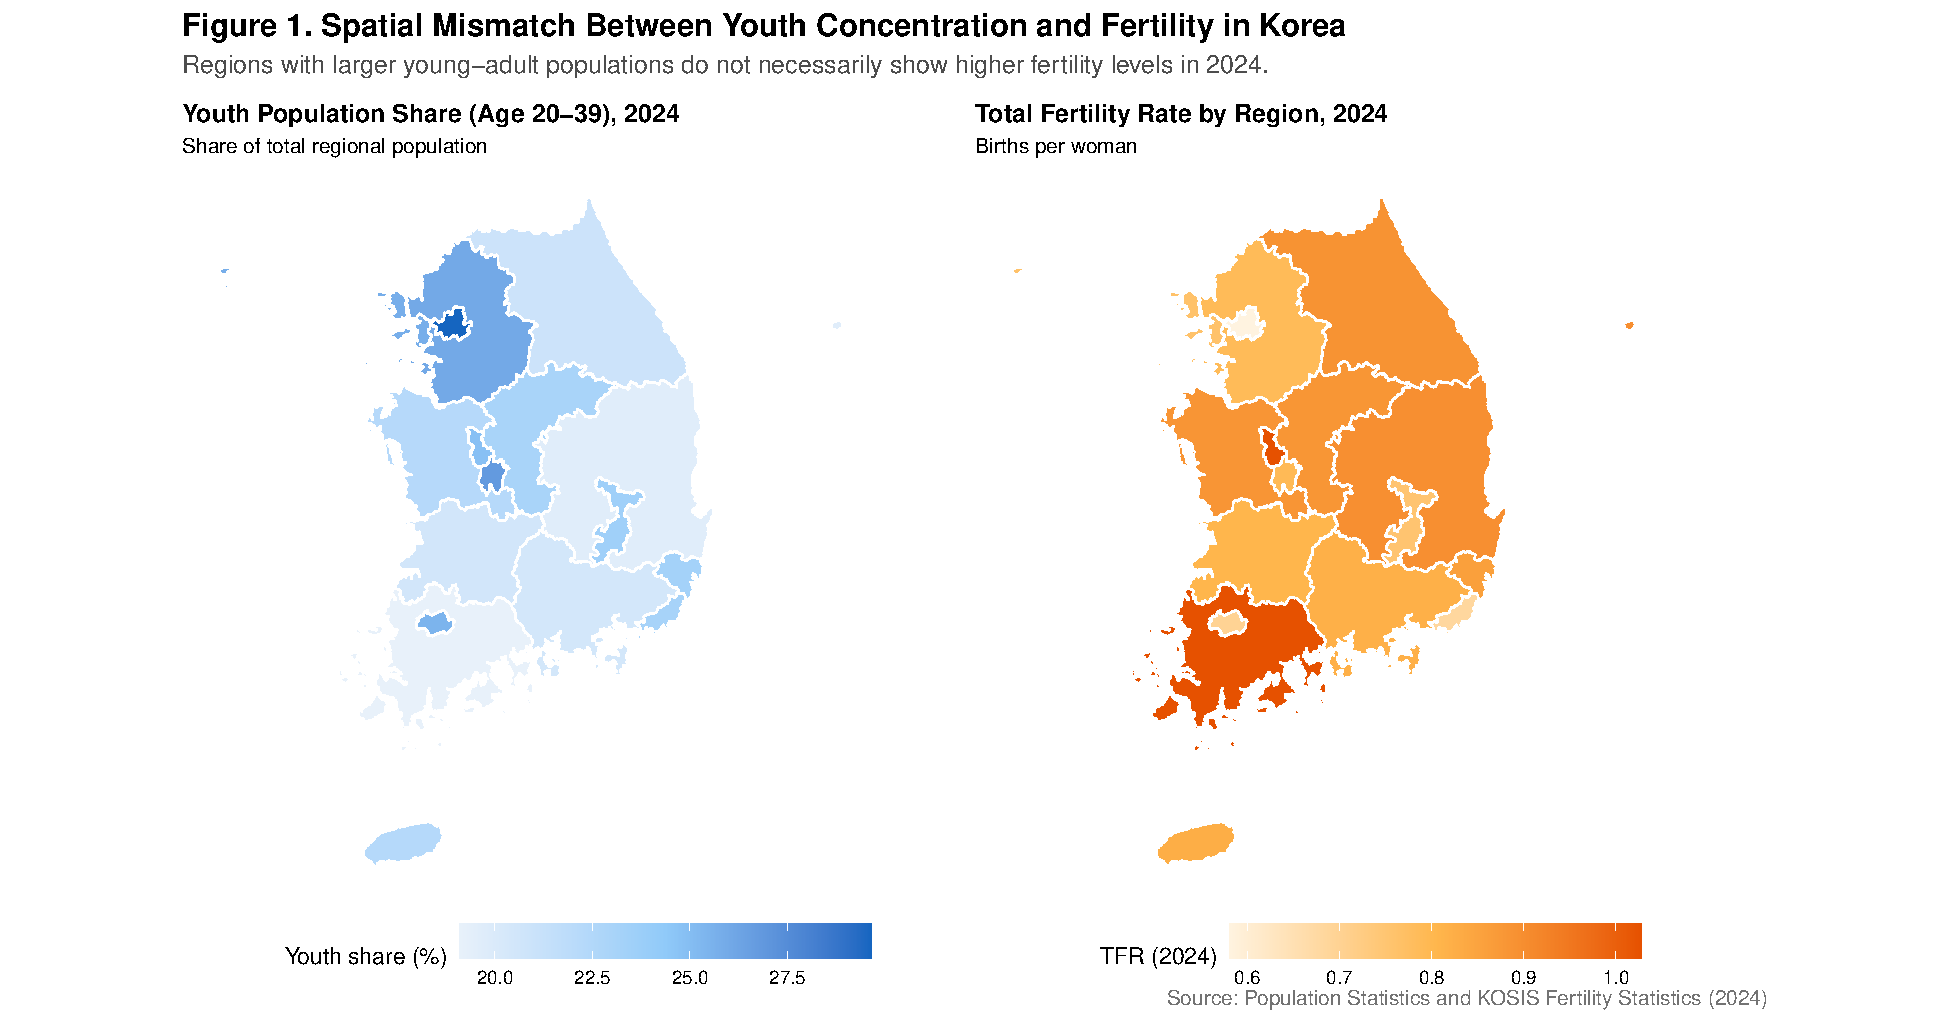
\includegraphics[width=\textwidth]{fig1.pdf}
		\caption{Side-by-side comparison of Youth Concentration and Fertility}
		\label{fig:figure1}
	\end{figure}
	
\subsubsection*{1) Explanation}
This visualization highlights a spatial pattern that may be interpreted as a \textbf{“Youth Black Hole”} phenomenon in Korea’s demographic landscape. Contrary to conventional wisdom, the Seoul Metropolitan Area---which has the highest concentration of the primary childbearing population (ages 20--39)---paradoxically records the lowest fertility rates in the nation. One possible interpretation is that intense urban concentration and competition in metropolitan regions may influence family formation decisions, potentially leading young adults to delay or reconsider starting a family. This figure suggests that regional imbalance is an important part of Korea’s low-fertility pattern.

\subsubsection*{2) Description}
\begin{itemize}
  \item \textbf{Map Composition:} This is a side-by-side choropleth map of South Korea's 17 administrative provinces. The left map represents the \textbf{Youth Population Share} (the ratio of the 20--39 age group to the total population), while the right map shows the \textbf{2024 Total Fertility Rate (TFR)}.
  \item \textbf{Color Encoding:} In the youth-share map (left), darker blue indicates a higher concentration of young adults. In the TFR map (right), darker orange/red indicates a higher fertility rate.
  \item \textbf{Key Interpretation:} The core of the analysis lies in identifying the \textbf{Spatial Mismatch}: the Seoul and Gyeonggi regions, which appear in the darkest blue on the left, appear in the lightest shades (lowest values) on the fertility map on the right.
\end{itemize}
	
	\subsubsection*{3) R code}
	\inputminted[firstline=144, lastline=188, breaklines=true, fontsize=\footnotesize, bgcolor=backcolour]{r}{finalproject_SK.R}
	
	
	
	\newpage
\subsection{Figure 2: Statistical Correlation Between Youth Share and Regional Fertility}
	\begin{figure}[H]
		\centering
		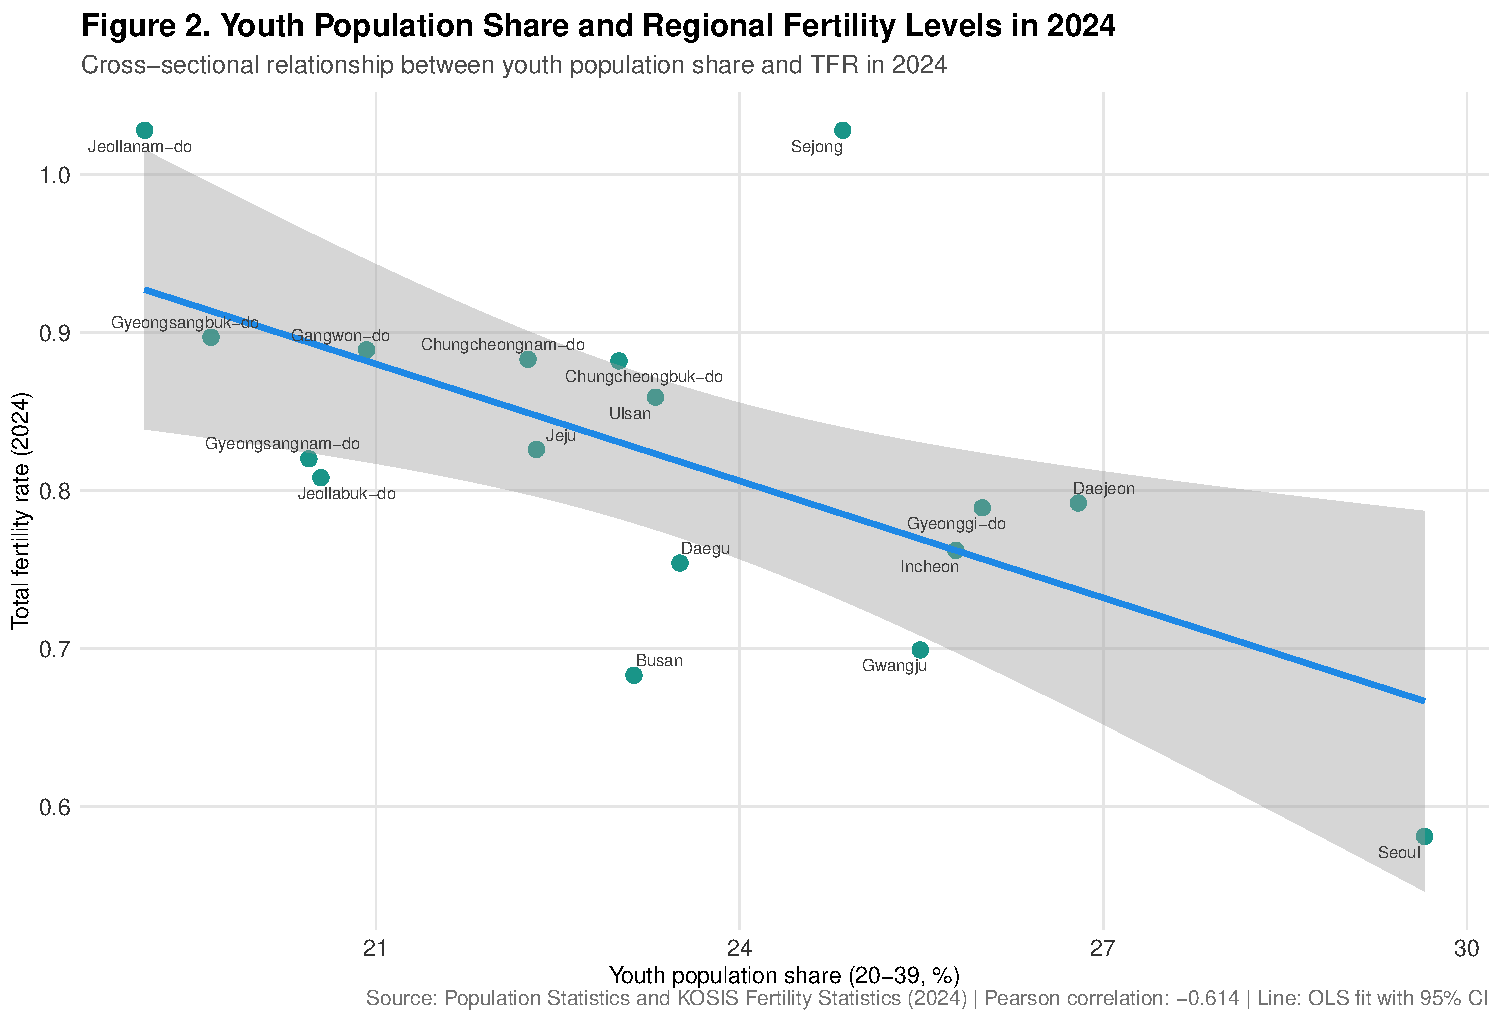
\includegraphics[width=0.9\textwidth]{fig2.pdf}
		\caption{Relationship between Youth Share and Regional Fertility}
		\label{fig:figure2}
	\end{figure}
	
\subsubsection*{1) Explanation}
To statistically verify the spatial paradox captured in Figure 1, a scatter-plot analysis combined with a regression model was conducted. A Pearson correlation coefficient of approximately -0.61 indicates a noticeable negative relationship:  regions with a higher share of young adults tend to have lower fertility rates. This pattern is consistent with the idea that metropolitan regions attract young adults through economic and educational opportunities. For young adults, the resulting competitive pressure may act as a \textbf{``push factor"} associated with delayed family formation and lower fertility outcomes.

\subsubsection*{2) Description}
\begin{itemize}
  \item \textbf{Axes:} The X-axis represents regional youth population share (\%), and the Y-axis represents the 2024 total fertility rate.
  \item \textbf{Regression Line \& Confidence Interval:} The blue straight line is the Ordinary Least Squares (OLS) regression line, and the surrounding grey area represents the 95\% confidence interval. The downward slope clearly suggests the inverse relationship between youth density and fertility.
  \item \textbf{Data Points:} Each regional data point is labeled using the \texttt{ggrepel} package. This allows a clear contrast between outliers like \texttt{Seoul} (highest youth share, lowest TFR) and regions like \texttt{Jeollanam-do} (lower youth share, relatively higher TFR).
\end{itemize}
	
	\subsubsection*{3) R code}
	\inputminted[firstline=190, lastline=210, breaklines=true, fontsize=\footnotesize, bgcolor=backcolour]{r}{finalproject_SK.R}
	
	
	
	\newpage
\subsection{Figure 3: Parallel Decline of Marriage and Fertility and the Echo Effect}
	\begin{figure}[H]
		\centering
		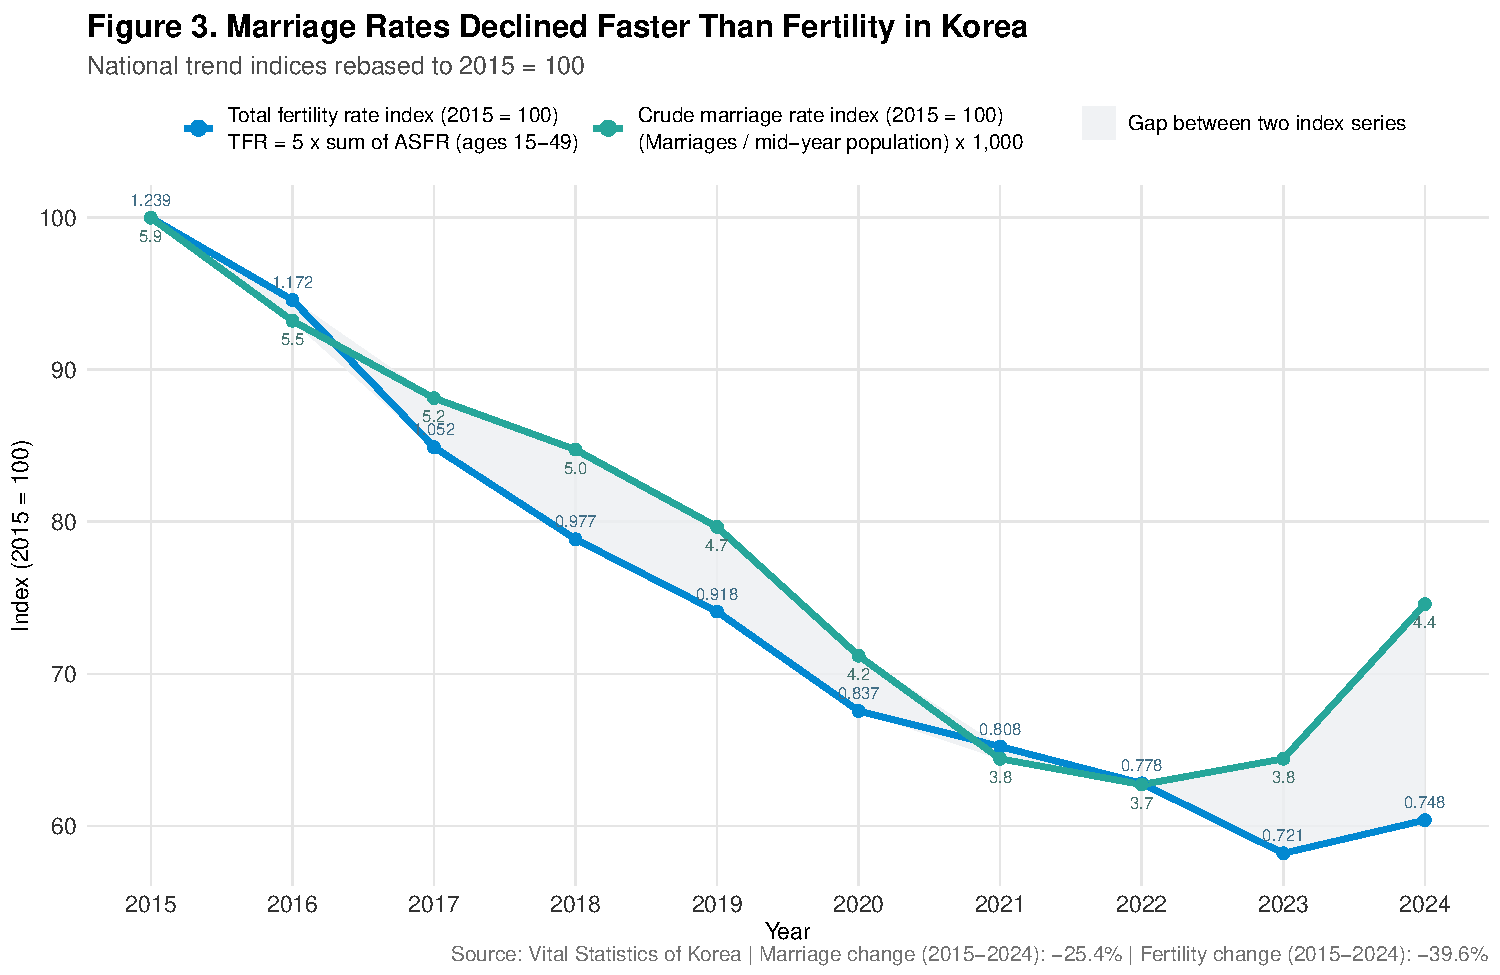
\includegraphics[width=0.9\textwidth]{fig3.pdf}
		\caption{Indexed Trends of Marriage and Fertility}
		\label{fig:figure3}
	\end{figure}
	
\subsubsection*{1) Explanation}
This figure analyzes the time-series coupling of marriage and childbirth to understand the underlying mechanics of the crisis. Given South Korea's unique sociocultural context---where the rate of out-of-wedlock births is exceptionally low compared to OECD averages---the marriage rates often move closely with fertility trends in the Korean context. The analysis shows that both indicators follow a parallel downward trajectory. Notably, the subtle uptick observed between 2022 and 2024 may not necessarily indicate a structural recovery. Instead, it may reflect what is sometimes described as a \textbf{“demographic echo”} effect caused by the 1990s cohort (the children of the second baby boomers) entering their peak marriageable age. This suggests that recent fluctuations may partly reflect cohort dynamics driven by population size rather than a fundamental behavioral shift.

\subsubsection*{2) Description}
\begin{itemize}
  \item \textbf{Indexing (Rebasing):} To compare two indicators with different units directly, the Y-axis uses a relative index with 2015 values set to 100.
  \item \textbf{Colors \& Lines:} The blue line represents the TFR index, and the green line represents the crude marriage-rate index. Their synchronized decline is consistent with the interpretation that retreat from marriage is an important component of the fertility crisis.
  \item \textbf{Ribbon \& Annotations:} The grey ribbon indicates the gap between decline rates of the two series. Raw observed values (TFR and marriage rate) are annotated near each data point, enabling simultaneous interpretation of rebased trends and absolute statistics.
\end{itemize}
	
	\subsubsection*{3) R code}
	\inputminted[firstline=212, lastline=270, breaklines=true, fontsize=\footnotesize, bgcolor=backcolour]{r}{finalproject_SK.R}
	
	
	
\end{document}
